\documentclass[10pt]{article}
\usepackage{theme}
\usepackage{shortcuts}
\usepackage{subcaption}
\setlength{\columnsep}{18pt}

\title{Mini-Project (ML for Time Series) -- Reproducing ``Riding Wavelets''}
\author{
Janis Aiad \email{janisaiad.ja@gmail.com} \\ % student 1
Jordi Baroja Fernandez \email{baroja.jordi@gmail.com} % student 2
}

\begin{document}
\maketitle

\section{Introduction and contributions}

Financial markets exhibit intermittent extreme events (``jumps'') that can be induced by external information (exogenous) or by internal feedback loops (endogenous). Aubrun et al. propose an unsupervised pipeline to classify jump time-series using wavelet-based features that capture multi-scale time-asymmetry of volatility, and show that two additional interpretable directions emerge: mean-reversion and trend.

We reproduced the core methodology end-to-end in Python, using open (Stooq) intraday OHLC data, and validated that the main qualitative conclusions are robust across markets (Poland and Hong Kong) and across data regimes.

\paragraph{Repartition of work, code reuse, experiments, improvements.}
\begin{itemize}
    \item \textbf{Work split.} Janis implemented the data curation, jump detection, ablations (threshold, time scale) and result aggregation; Jordi implemented wavelet variants and robustness checks (kernel choices, scale parameter $J$) and plotting utilities.
    \item \textbf{Code reuse.} No public codebase was available for the full pipeline; we implemented the complete methodology ourselves using standard libraries (\texttt{numpy}, \texttt{pandas}, \texttt{PyWavelets}, \texttt{scikit-learn}). 
    \item \textbf{New experiments.} We ran ablations on (i) inclusion/exclusion of Scattering Spectra features, (ii) wavelet scales $J$, (iii) threshold choice, and (iv) multiple markets.
    \item \textbf{Improvements.} We packaged the wavelet feature extraction and Kernel PCA in a reusable module and ensured reproducibility on open data.
\end{itemize}

\section{Method}

\subsection{Jump detection}
For each asset we compute returns $r(t)$ and a de-seasonalized local volatility estimate $f(t)\sigma(t)$, then define the standardized return profile:
\[
x(t) = \frac{r(t)}{f(t)\sigma(t)}.
\]
Jumps are detected when $|x(t)|>\theta$ with $\theta=4$ in the base setting. We exclude the first and last hour of each trading day to mitigate open/close microstructure effects.

\paragraph{Non-stationarity and volatility normalization.}
Raw returns exhibit volatility clustering and time-varying scales, so learning global templates (e.g., dictionary learning) or relying on naive stationarity assumptions is brittle. We therefore de-seasonalize intraday patterns via $f(t)$ and normalize by a local volatility estimate $\sigma(t)$ to construct the standardized score $x(t)$ used for jump detection. For daily data, $\sigma(t)$ can be noisier but stabilizes with longer spans.

\subsection{Wavelet scattering features and interpretable directions}
For each detected jump, we extract a window $x(t)$ centered at the jump time $t=0$ and use the jump-aligned profile $\overline{x}(t)=\mathrm{sign}(x(0))\,x(t)$ so that all jumps have positive center return.

We implement the wavelet scattering representation:
\[
\Phi(x) = \big(W_j \overline{x}(0),\; W_{j_2}\,|W_{j_1}x|(0)\big)_{1\le j \le J,\; 1\le j_1 < j_2\le J},
\]
where $W_j$ denotes the complex wavelet transform at dyadic scale $2^j$. We concatenate real and imaginary parts and normalize coefficients by scale energy to reduce sensitivity to amplitude.

Kernel PCA with an RBF kernel applied to standardized $\Phi(x)$ produces an embedding whose first component $D_1$ is expected to measure time-asymmetry of volatility (``reflexivity'' direction). We also compute two local, interpretable scalar scores from the centered window:
\[
D_2 = x(-1) - x(+1),\qquad D_3 = x(-1) + x(+1),
\]
which capture short-term mean-reversion and trend alignment around the jump.

\subsection{Scattering Spectra (ablation)}
We optionally augment $\Phi(x)$ with Scattering Spectra (SS) features (low-order moments of wavelet coefficients across scales) to test whether they provide additional information beyond wavelet scattering coefficients.

\section{Data}

We use open source \href{https://stooq.com}{Stooq} OHLC data for multiple stock markets and multiple sampling frequencies (5-min, hourly, daily; see Tables~\ref{tab:data_poland} and~\ref{tab:data_hungary}). Since the original paper uses 1-minute data with a 119-point window and $J=6$, we adapt to coarser bars with shorter windows and set $J=3$ for 5-min experiments.

\begin{table*}[t]
\centering
\scriptsize
\setlength{\tabcolsep}{4pt}
\renewcommand{\arraystretch}{1.15}
\begin{tabular}{lrrrll}
\toprule
freq & $n$ stocks & total points & span (days) & start & end \\
\midrule
5min   & 80 & 477302 & 148   & 07/07/2025 10:00 & 12/02/2025 15:40 \\
hourly & 80 & 105700 & 628   & 04/11/2024 11:00 & 12/30/2025 16:00 \\
daily  & 80 & 254918 & 10205 & 01/21/1998       & 12/30/2025 \\
\bottomrule
\end{tabular}
\caption{Poland dataset summary (after preprocessing).}
\label{tab:data_poland}
\end{table*}

\begin{table*}[t]
\centering
\scriptsize
\setlength{\tabcolsep}{4pt}
\renewcommand{\arraystretch}{1.15}
\begin{tabular}{lrrrll}
\toprule
freq & $n$ stocks & total points & span (days) & start & end \\
\midrule
5min   & 23 &  52081 & 147   & 06/10/2025 10:00 & 11/04/2025 15:55 \\
hourly & 35 &  44143 & 572   & 04/11/2024 11:00 & 11/04/2025 16:00 \\
daily  & 30 & 109233 & 11849 & 05/27/1993       & -- \\
\bottomrule
\end{tabular}
\caption{Hungary dataset summary (after preprocessing).}
\label{tab:data_hungary}
\end{table*}

\subsection*{Preprocessing diagnostics: jump-score distribution and tails}
The standardized returns exhibit heavy tails; the upper tail of $|x(t)|$ is well captured by a Gumbel fit on a high-quantile range, consistent with the max-stable null model discussed in the paper. We aggregate 12$\times$5-min bars into hourly and 12$\times$hourly into daily; since the number of observations (and thus extreme events) decreases sharply at coarser scales, we use lower practical thresholds at coarser frequencies (roughly $\theta\approx4$ for 5-min, $\theta\approx3$ for hourly, $\theta\approx2$ for daily) to retain enough jumps for stable statistics. We note that the 5-min tail shows a mild deviation from the Gumbel fit in the far tail; this could indicate a heavier-than-exponential tail (suggesting a Fr\'echet/GEV-type behavior) rather than a pure Gumbel regime, but we do not push this interpretation further here. We also note that our volatility estimator was adjusted during development; a deeper extreme-value analysis (e.g., GEV/GPD fits on exceedances) is left for future work.

\begin{figure}[H]
\centering
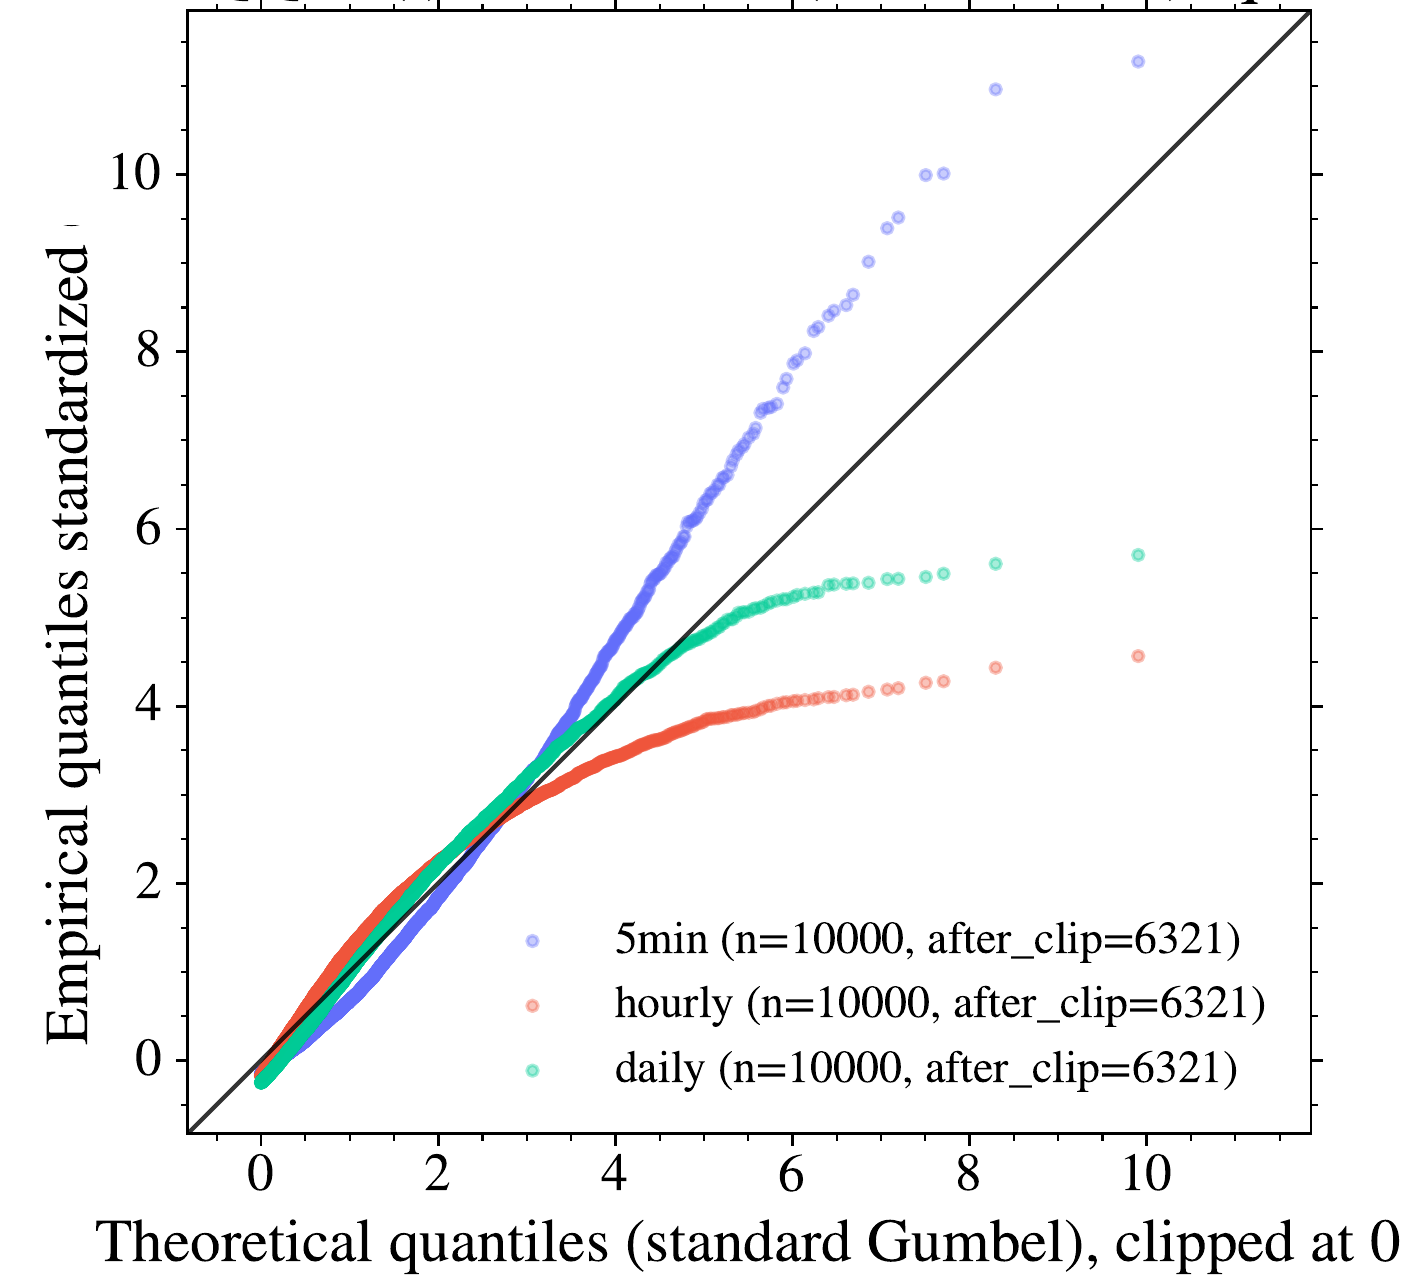
\includegraphics[width=0.35\linewidth]{figures/2/qq_abs_score_vs_gumbel_STACKED_mpl.png}
\caption{Q--Q plot of $|x(t)|$ against the fitted Gumbel distribution (stacked across 5-min, hourly, daily).}
\label{fig:poland_gumbel}
\end{figure}

\begin{figure*}[t]
\centering
\begin{subfigure}{0.48\textwidth}
    \centering
    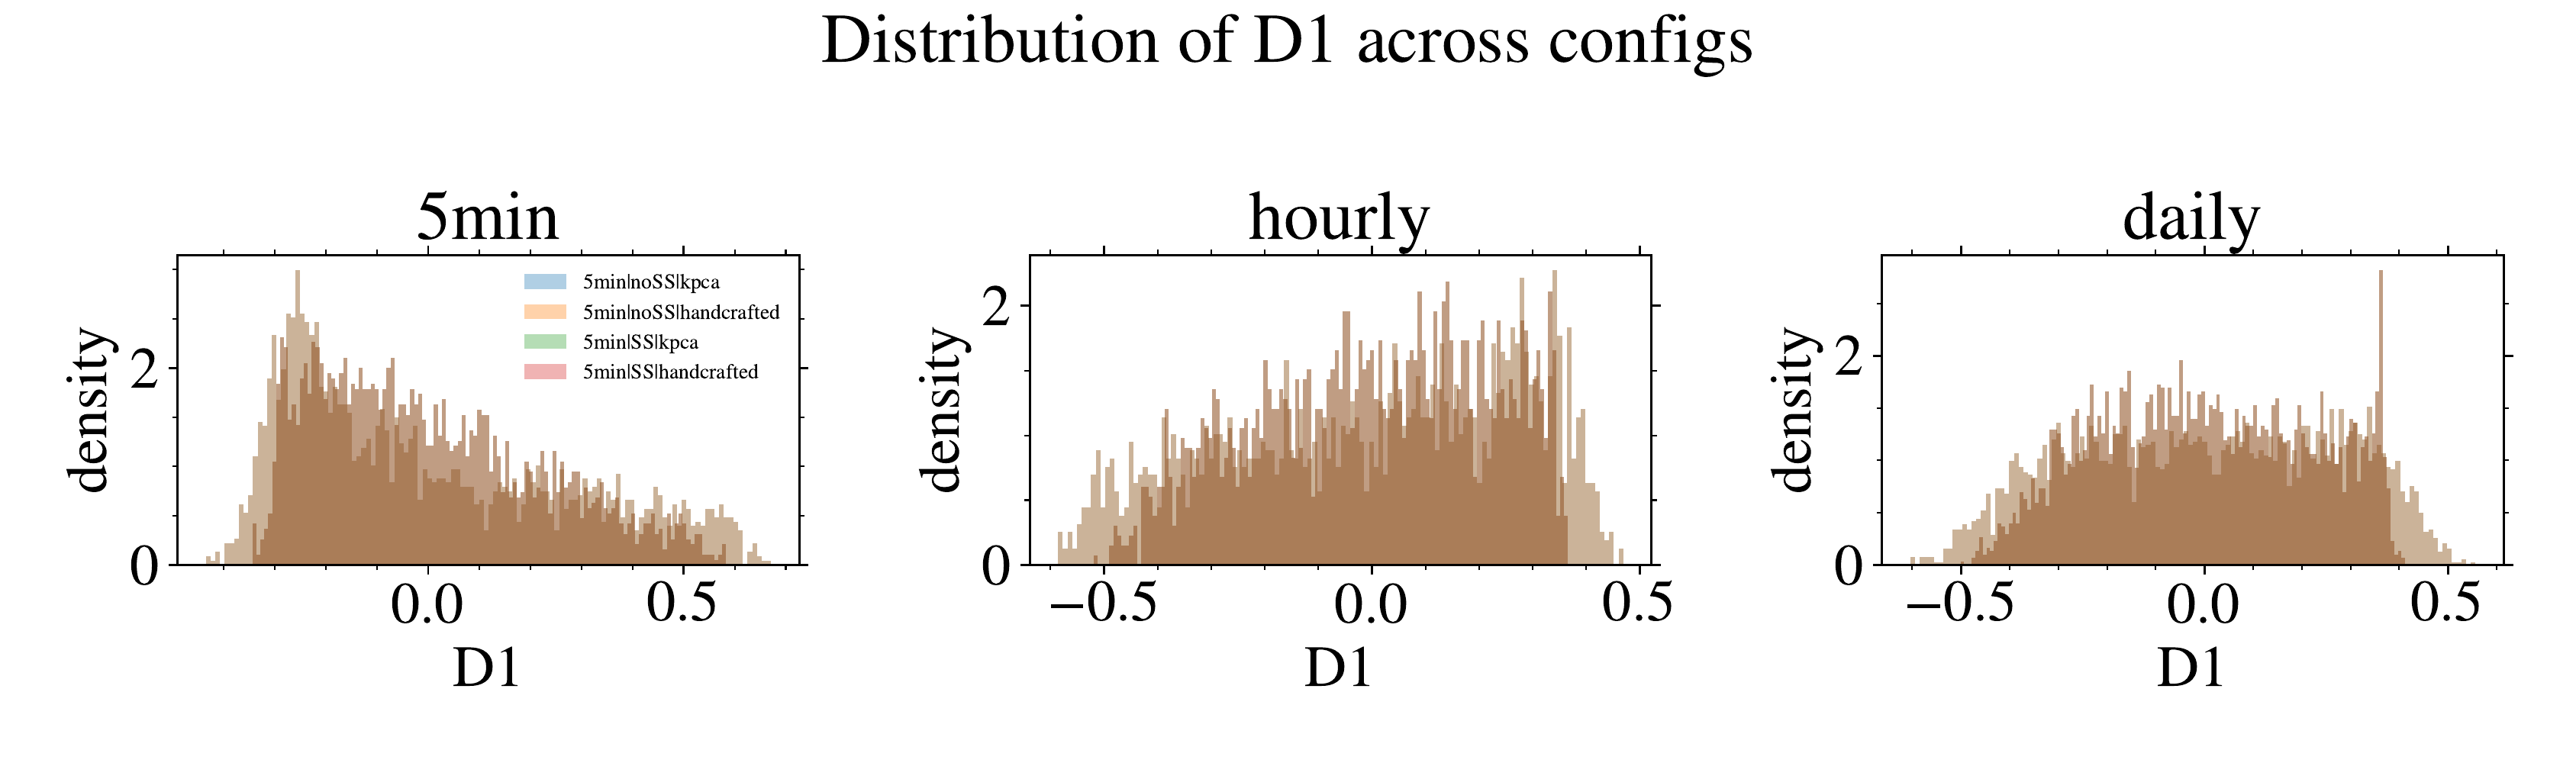
\includegraphics[width=\textwidth]{figures/2/hist_D1_mpl.png}
    \caption{Distribution of $D_1$ (linear scale).}
\end{subfigure}
\begin{subfigure}{0.48\textwidth}
    \centering
    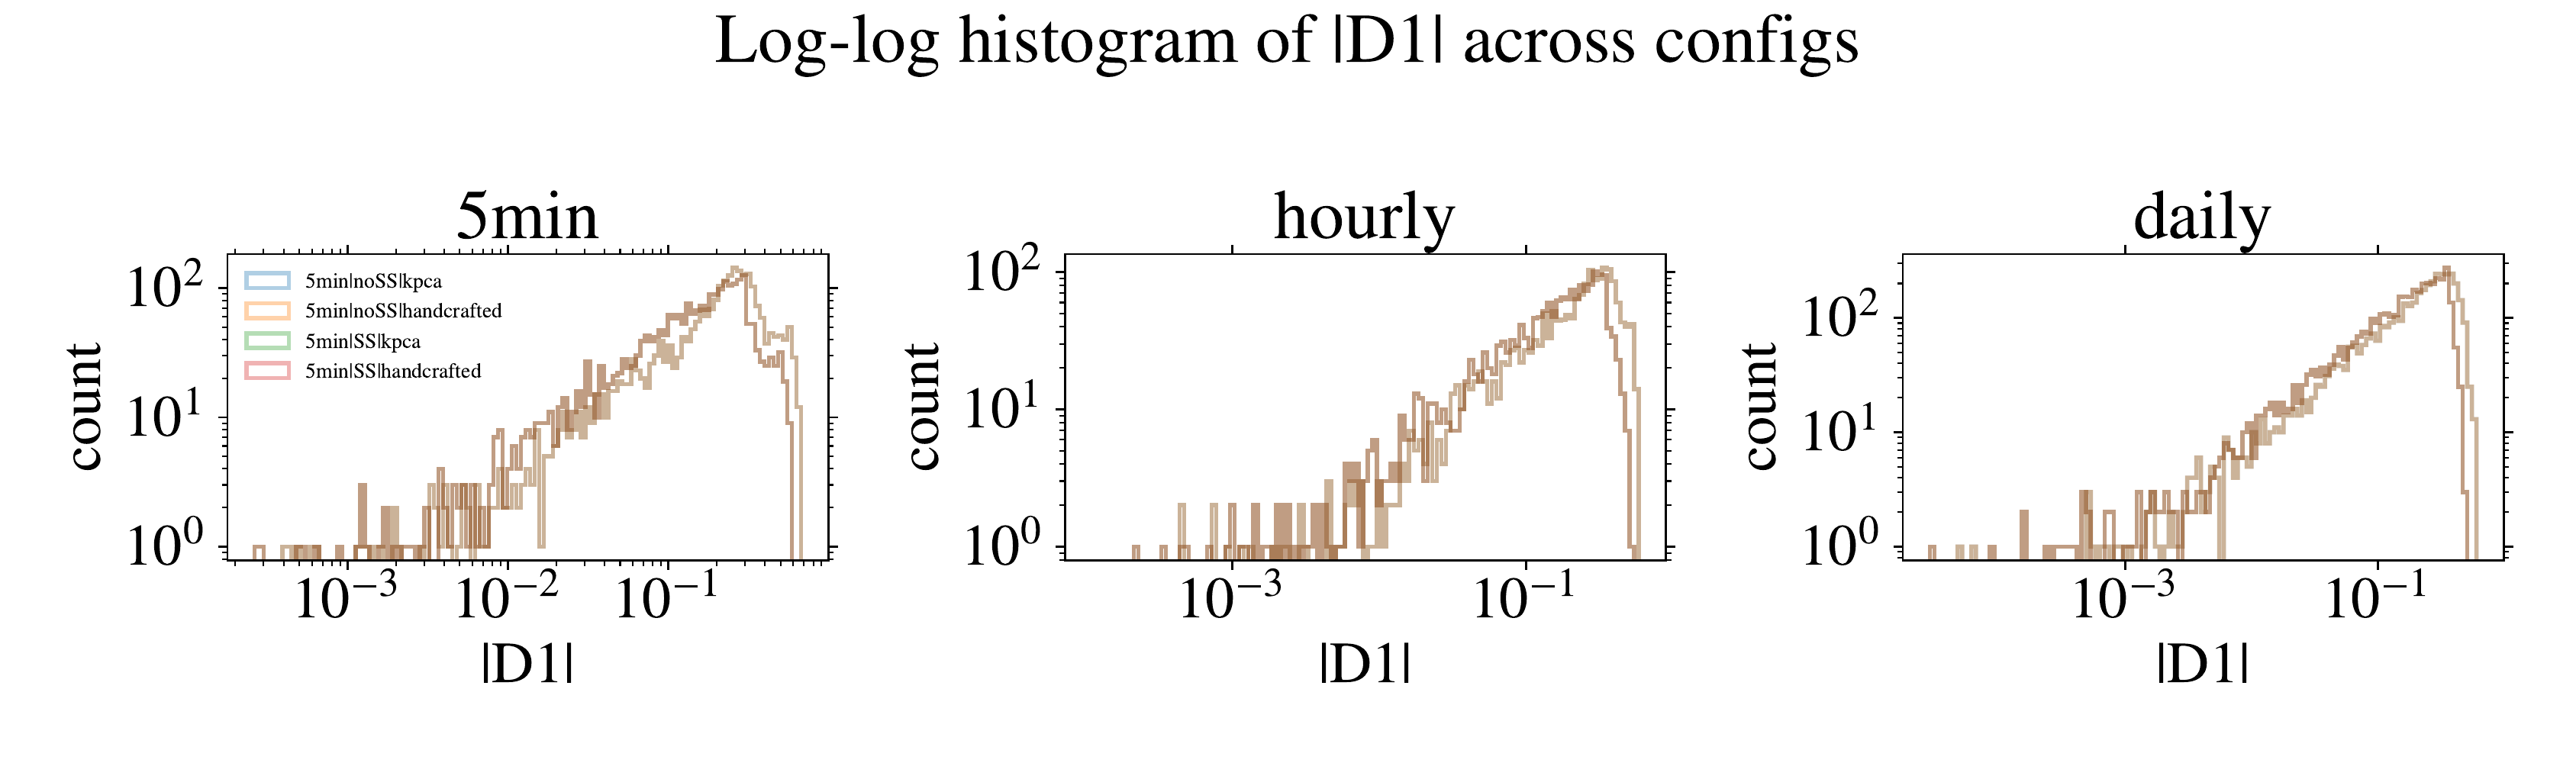
\includegraphics[width=\textwidth]{figures/2/hist_abs_loglog_D1_mpl.png}
    \caption{Distribution of $|D_1|$ (log--log).}
\end{subfigure}
\begin{subfigure}{0.48\textwidth}
    \centering
    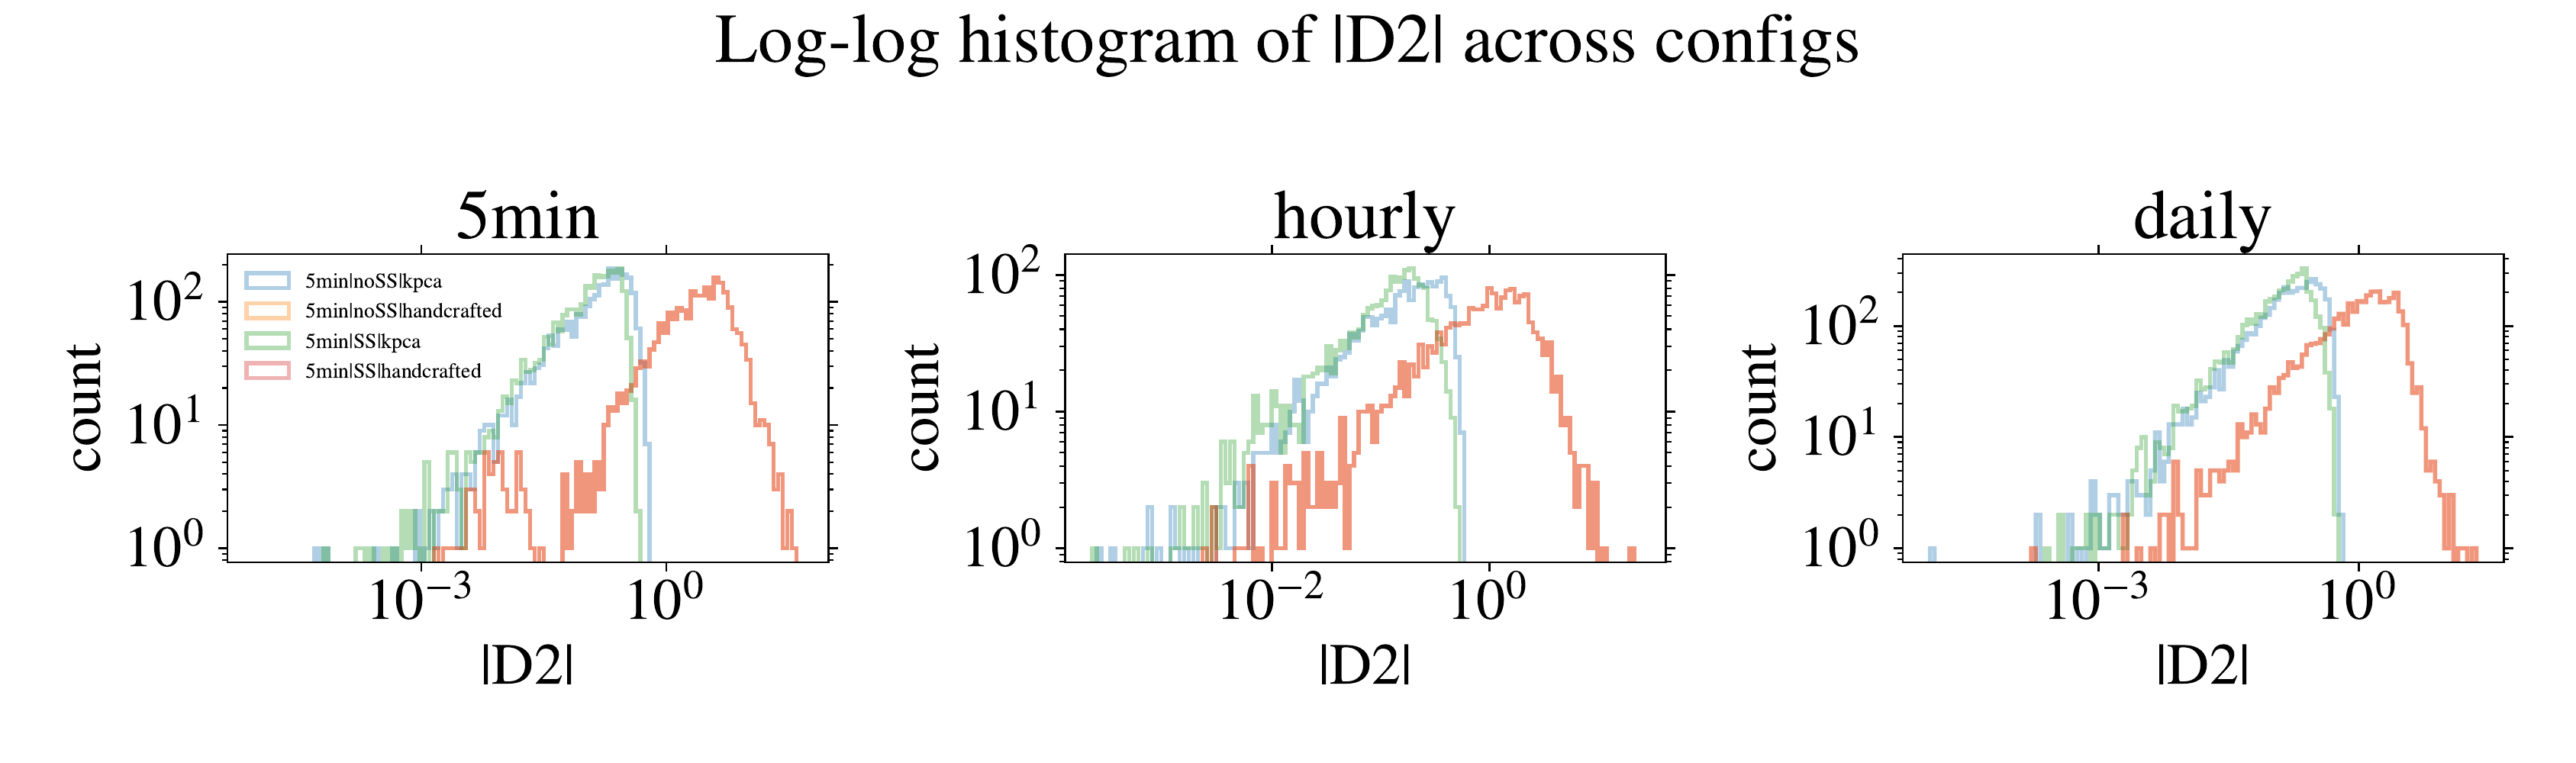
\includegraphics[width=\textwidth]{figures/2/hist_abs_loglog_D2_mpl.png}
    \caption{Distribution of $|D_2|$ (log--log).}
\end{subfigure}
\begin{subfigure}{0.48\textwidth}
    \centering
    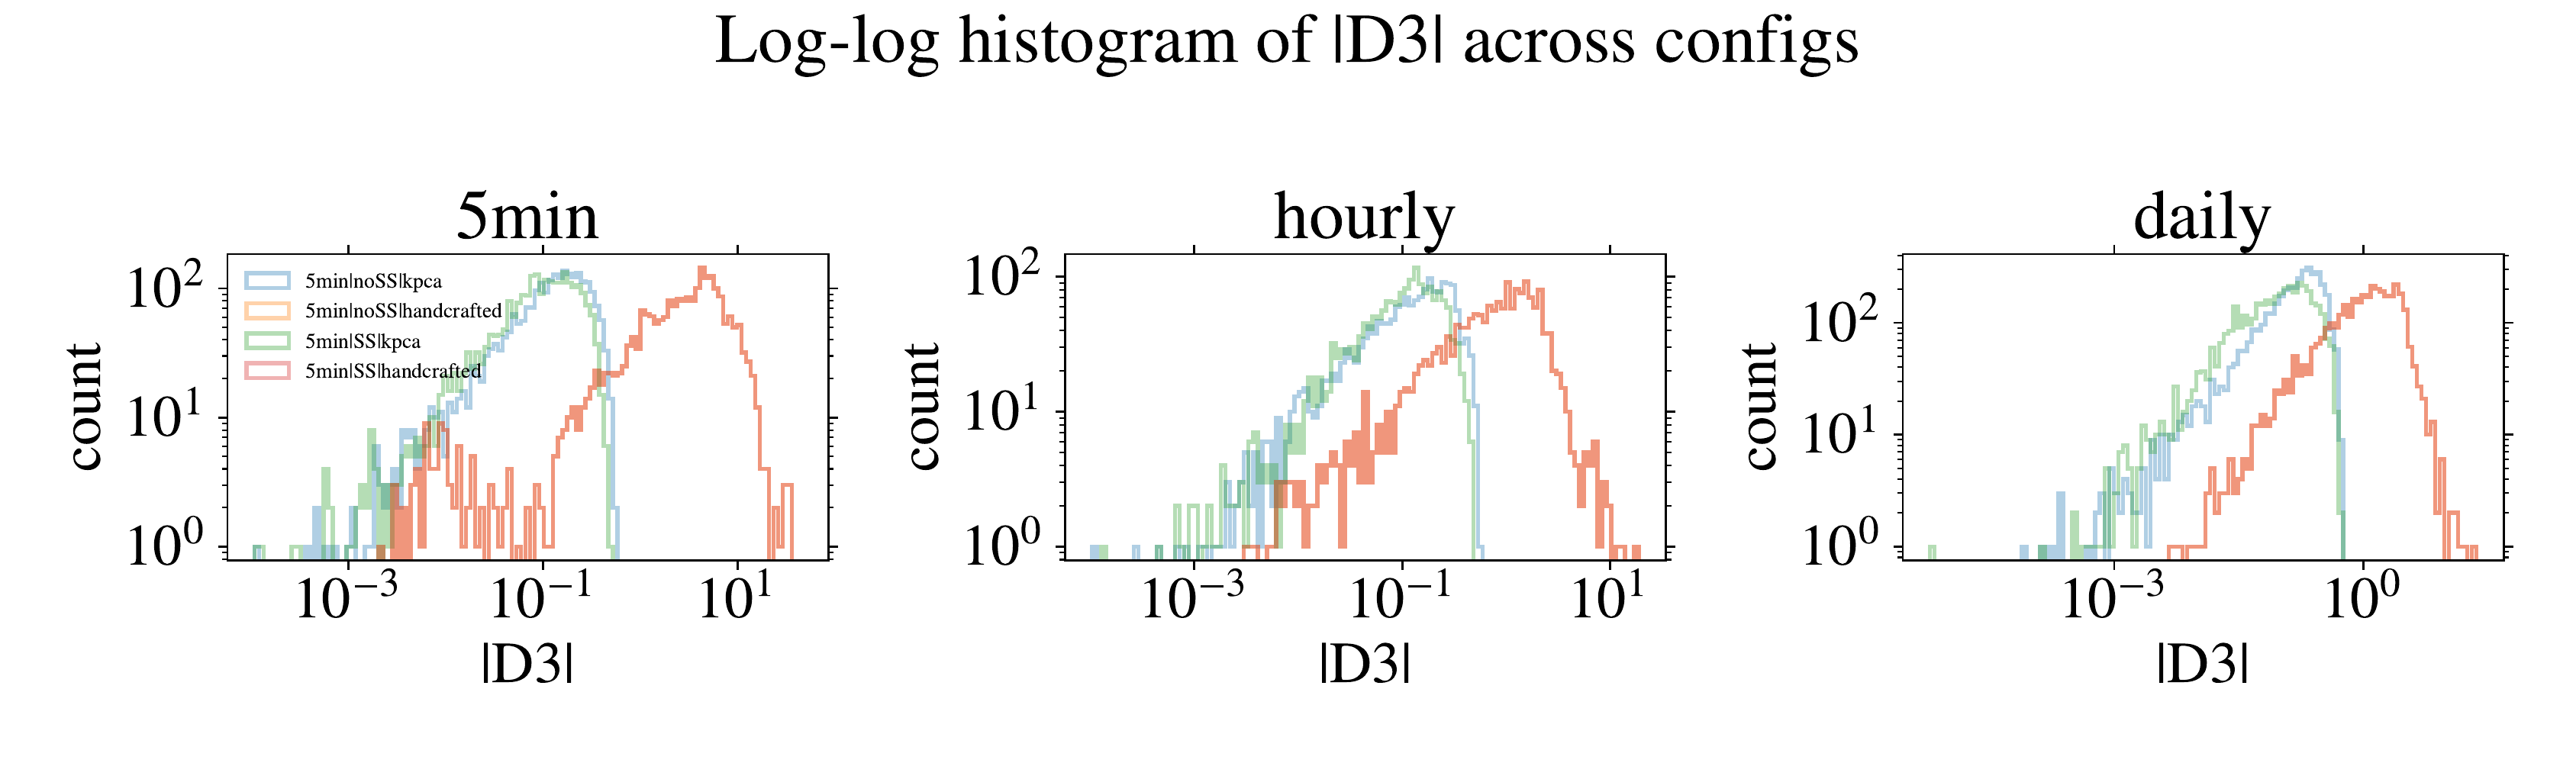
\includegraphics[width=\textwidth]{figures/2/hist_abs_loglog_D3_mpl.png}
    \caption{Distribution of $|D_3|$ (log--log).}
\end{subfigure}
\caption{Distribution diagnostics (Poland, 5-min): reflexivity score $D_1$ and tails of $|D_1|,|D_2|,|D_3|$.}
\label{fig:score_distributions}
\end{figure*}

\paragraph{Data conclusion.}
Overall, the preprocessing checks support the hypotheses needed for the wavelet pipeline: after de-seasonalization and volatility normalization, jump scores have stable heavy-tail behavior compatible with the paper's extreme-value motivation, and the learned directions exhibit well-behaved empirical distributions. This gives confidence that applying the embedding and interpretability analysis below is meaningful on our datasets.

\section{Results}

\subsection{Recovered directions: reflexivity, mean-reversion, trend}
We recover the key qualitative structure of the paper: $D_1$ captures volatility time-asymmetry (reflexivity), while $D_2$ and $D_3$ capture short-term mean-reversion and trend behaviors. The distributional diagnostics for $|x(t)|$ (Gumbel Q--Q) and for the learned scores ($D_1$ and the tails of $|D_1|,|D_2|,|D_3|$) are reported in the Data section as preprocessing checks.

Projecting onto $(D_1,D_2)$ and $(D_1,D_3)$ separates interpretable behaviors (mean-reversion and trend). Due to the strict page limit and focus on robustness, we report the 2D projections qualitatively and focus on the score distributions and threshold sweeps shown below.

\subsection{Ablation: Scattering Spectra features}
Adding SS features yields very similar $D_1$ embeddings (high correlation), suggesting that the base wavelet scattering coefficients already capture the dominant reflexivity signal at this resolution. Due to the strict page limit, we report this ablation qualitatively in text and keep the threshold-robustness figure below.

\subsection{Robustness to the jump threshold (5-min)}
We evaluate the sensitivity of the discovered directions to the jump-detection threshold $\theta$. For 5-min data, we observe a striking stability across thresholds (e.g., $\theta\in[2.5,4.5]$): $D_1$ and $D_3$ profiles are nearly unchanged, while $D_2$ can degrade slightly at the most extreme thresholds due to a small set of outliers that do not follow the typical mean-reversion pattern.
Supplementary overlays for hourly and daily data are provided in \texttt{refs/report/mva\_appendix.pdf}.

\begin{figure*}[t]
\centering
\begin{subfigure}{0.32\textwidth}
    \centering
    
\includegraphics[width=\textwidth]{figures/2/overlay_D1_thresholds_5min_mpl.png}
    \caption{$D_1$ overlays.}
\end{subfigure}
\begin{subfigure}{0.32\textwidth}
    \centering
    
\includegraphics[width=\textwidth]{figures/2/overlay_D2_thresholds_5min_mpl.png}
    \caption{$D_2$ overlays.}
\end{subfigure}
\begin{subfigure}{0.32\textwidth}
    \centering
    
\includegraphics[width=\textwidth]{figures/2/overlay_D3_thresholds_5min_mpl.png}
    \caption{$D_3$ overlays.}
\end{subfigure}
\caption{Threshold sweep (5-min): average profiles along $D_1$, $D_2$, $D_3$ remain qualitatively stable across thresholds.}
\label{fig:threshold_sweep_5min}
\end{figure*}

\paragraph{Conclusion.}
Our reproduction confirms that wavelet-based embeddings recover interpretable jump classes, with $D_1$ measuring volatility time-asymmetry and complementary mean-reversion/trend directions emerging from local signed profiles. On our open-data setting, Scattering Spectra features do not materially change the main reflexivity direction.

\begin{thebibliography}{9}
\bibitem{aubrun_ridingwavelets}
C.~Aubrun, R.~Morel, M.~Benzaquen, and J.-P.~Bouchaud.
\newblock Riding wavelets: A method to discover new classes of price jumps.
\newblock (preprint / manuscript version in \texttt{refs/texsources/ridingwavelets}).

\bibitem{bruna_mallat}
J.~Bruna and S.~Mallat.
\newblock Invariant scattering convolution networks.
\newblock \emph{IEEE Transactions on Pattern Analysis and Machine Intelligence}, 35(8):1872--1886, 2013.

\bibitem{morel_scatteringspectra}
R.~Morel et al.
\newblock Scattering spectra for scale-invariant time series analysis.
\newblock (see references in the original paper).
\end{thebibliography}



\section*{Appendix: Threshold sweep overlays across frequencies}

This supplementary appendix provides the full set of threshold-sweep overlay plots across sampling frequencies (5-min, hourly, daily) for the three main directions ($D_1$, $D_2$, $D_3$). The main report includes the 5-min overlays; the plots below show the complete comparison grid.

\begin{figure}[H]
\centering
\begin{subfigure}{0.32\textwidth}
    \centering
    
\includegraphics[width=\textwidth]{figures/2/overlay_D1_thresholds_5min_mpl.png}
    \caption{$D_1$ (5-min)}
\end{subfigure}
\begin{subfigure}{0.32\textwidth}
    \centering
    
\includegraphics[width=\textwidth]{figures/2/overlay_D1_thresholds_hourly_mpl.png}
    \caption{$D_1$ (hourly)}
\end{subfigure}
\begin{subfigure}{0.32\textwidth}
    \centering
    
\includegraphics[width=\textwidth]{figures/2/overlay_D1_thresholds_daily_mpl.png}
    \caption{$D_1$ (daily)}
\end{subfigure}

\begin{subfigure}{0.32\textwidth}
    \centering
    
\includegraphics[width=\textwidth]{figures/2/overlay_D2_thresholds_5min_mpl.png}
    \caption{$D_2$ (5-min)}
\end{subfigure}
\begin{subfigure}{0.32\textwidth}
    \centering
    
\includegraphics[width=\textwidth]{figures/2/overlay_D2_thresholds_hourly_mpl.png}
    \caption{$D_2$ (hourly)}
\end{subfigure}
\begin{subfigure}{0.32\textwidth}
    \centering
    
\includegraphics[width=\textwidth]{figures/2/overlay_D2_thresholds_daily_mpl.png}
    \caption{$D_2$ (daily)}
\end{subfigure}

\begin{subfigure}{0.32\textwidth}
    \centering
    
\includegraphics[width=\textwidth]{figures/2/overlay_D3_thresholds_5min_mpl.png}
    \caption{$D_3$ (5-min)}
\end{subfigure}
\begin{subfigure}{0.32\textwidth}
    \centering
    
\includegraphics[width=\textwidth]{figures/2/overlay_D3_thresholds_hourly_mpl.png}
    \caption{$D_3$ (hourly)}
\end{subfigure}
\begin{subfigure}{0.32\textwidth}
    \centering
    
\includegraphics[width=\textwidth]{figures/2/overlay_D3_thresholds_daily_mpl.png}
    \caption{$D_3$ (daily)}
\end{subfigure}

\caption{Threshold sweep overlays across frequencies (5-min, hourly, daily).}
\label{fig:threshold_sweep_all}
\end{figure}

\end{document}



\end{document}


